% =============================================================================
% 4IT218 Databáze – Semestrální práce
% Platforma na publikování a sledování amatérských filmů
% =============================================================================
\documentclass[12pt,a4paper]{article}

\usepackage[utf8]{inputenc}
\usepackage[T1]{fontenc}
\usepackage[czech]{babel}
\usepackage{geometry}
\geometry{a4paper, margin=2.5cm}
\usepackage{graphicx}
\usepackage{booktabs}
\usepackage{longtable}
\usepackage{tabularx}
\usepackage{array}
\usepackage{float}
\usepackage{hyperref}
\usepackage{xcolor}
\usepackage[inputencoding=utf8]{listings}
\usepackage{fancyhdr}
\usepackage{enumitem}
% TikZ removed -- conceptual schema is an external image
\usepackage{caption}

% SQL listing style
\lstdefinestyle{sql}{
  basicstyle=\ttfamily\small,
  breaklines=true,
  showstringspaces=false,
  frame=single,
  backgroundcolor=\color{gray!5},
  numbers=none,
  commentstyle=\itshape\color{green!50!black},
  morecomment=[l]{--},
  morecomment=[s]{/*}{*/}
}

\lstset{style=sql}

% Header/footer
\pagestyle{fancy}
\fancyhf{}
\fancyhead[L]{\small Katedra informačních technologií, FIS, VŠE v~Praze}
\fancyfoot[C]{\thepage}
\renewcommand{\headrulewidth}{0.4pt}
\setlength{\headheight}{13.86pt}

\begin{document}

% ---- TITLE PAGE ----
\begin{titlepage}
\centering
\vspace*{2cm}
{\LARGE\bfseries Platforma na publikování a sledování\\amatérských filmů\par}
\vspace{1cm}
{\Large Dokumentace semestrální práce pro předmět 4IT218 Databáze\par}
\vspace{1.5cm}
{\Large Filip Troníček\par}
\vspace{0.5cm}
{\Large 2025/2026, letní semestr\par}
\vspace{1cm}
{\large Uživatelské jméno: trof01\par}
\vfill
{\large Katedra informačních technologií, Fakulta informatiky a statistiky,\\
Vysoká škola ekonomická v~Praze\par}
\end{titlepage}

% ---- TABLE OF CONTENTS ----
\tableofcontents

\vfill
\noindent\textit{Dokumentace tabulek, integritních omezení a~datového obsahu byla zpracována
za pomoci Large Language Modelu Claude 4.6 Opus.}
\newpage

% ====================================================================
% 1. POPIS ZVOLENÉ VÝSEČE SVĚTA – ZADÁNÍ
% ====================================================================
\section{Popis zvolené výseče světa -- zadání}

Pro potřeby webové streamingové platformy zaměřené na nezávislou a~amatérskou filmovou tvorbu
je zapotřebí evidovat údaje o~uživatelích, kanálech, videích, a také jejich hodnoceních a~sledování.

\subsection*{Uživatelé a~autentizace}

O~každém \textbf{uživateli} se eviduje umělý unikátní identifikátor (\texttt{id}, UUID), jméno,
volitelná URL profilového obrázku (\texttt{avatar\_url}) a~role v~rámci platformy --
buď \emph{uzivatel}, nebo \emph{admin}\footnote{Tyto systémové role jsou odlišné od rolí, které uživatelům náleží přes členství u nějakého kanálu (viz sekce \hyperref[sec:memberships]{Kanály a~členství}).}.

Každý uživatel se přihlašuje prostřednictvím právě jednoho externího poskytovatele identity.
O~každém poskytovateli (\textbf{OAuth konfigurace}) se evidují: unikátní identifikátor
(\texttt{id}, UUID), název (unikátní v~rámci platformy), volitelná URL loga
(\texttt{logo\_url}), autorizační URL (\texttt{authorization\_url}), rozsahy oprávnění
(\texttt{scopes}), URL pro výměnu tokenu (\texttt{token\_url}), volitelná URL pro získání
informací o~uživateli (\texttt{user\_info\_url}), identifikátor klienta (\texttt{client\_id})
a~tajný klíč (\texttt{client\_secret}).

\subsection*{Kanály a~členství}
\label{sec:memberships}

Uživatelé organizují svůj obsah prostřednictvím \textbf{kanálů}. O~každém kanálu se eviduje
unikátní identifikátor (\texttt{id}, UUID), název a~volitelný slug (URL-friendly identifikátor\footnote{Viz \href{https://datatracker.ietf.org/doc/html/rfc4648\#section-5}{RFC 4648 §5}},
který -- pokud je uveden -- musí být v~rámci platformy unikátní).

Kanál může mít více členů a~jeden uživatel může být členem více kanálů (vztah M:N).
V~každém kanálu má uživatel přiřazenu právě jednu roli (např. \emph{admin}, \emph{clen}).

\subsection*{Videa}

Kanál publikuje \textbf{videa}. O~každém videu se eviduje unikátní identifikátor (\texttt{id},
UUID), název, volitelný popis, volitelné datum publikace, volitelná URL náhledového obrázku
(\texttt{nahledovy\_obrazek\_url}) a~volitelná URL na MPEG-DASH manifest\footnote{Volitelná je tato URL proto, že video ji při vytvoření nemusí mít. V praxi by videa, která jsou vskutku přehratelná, tuto URL mít měla.}
(\texttt{manifest\_url}). Každé video je vlastněno právě jedním kanálem.

\subsection*{Hodnocení videí}

Uživatelé mohou videa hodnotit. \textbf{Hodnocení} je vztahová entita mezi uživatelem a~videem
(M:N). O~každém hodnocení se eviduje počet hvězdiček (\texttt{pocet\_hvezdicek}, číselná
hodnota v~rozsahu 1 až 5, přičemž jsou povoleny i~poloviční hodnoty, např. 2,5), volitelný
textový komentář a~datum publikace hodnocení. Jeden uživatel může hodnotit jedno video
nejvýše jednou.

\subsection*{Sledování}

Platforma sleduje přehrávání videí od různých uživatelů. \textbf{Sledování} je vztahová entita
mezi uživatelem a~videem (M:N). Každý záznam o~sledování má vlastní unikátní identifikátor
(\texttt{id}, UUID), protože jeden uživatel může mít více záznamů o~sledování téhož videa
(např. opakované zhlédnutí nebo více heartbeatů v~rámci jednoho přehrávání).
Dále se zaznamenává čas začátku sledování (\texttt{cas\_od}, povinný, v~sekundách od
začátku videa), volitelný čas konce (\texttt{cas\_do}, v~sekundách) a~volitelný identifikátor
relace (\texttt{session\_id}, UUID).

\subsection*{Podporované dotazy}
\begin{itemize}
  \item Jaká videa patří ke konkrétnímu kanálu?
  \item Jak je dané video hodnoceno?
  \item Kdo je členem kanálu a~ jakou v~ něm má roli?
\end{itemize}

\newpage

% ====================================================================
% 2. KONCEPTUÁLNÍ SCHÉMA REALITY
% ====================================================================
\section{Konceptuální schéma reality}

\begin{figure}[H]
\centering
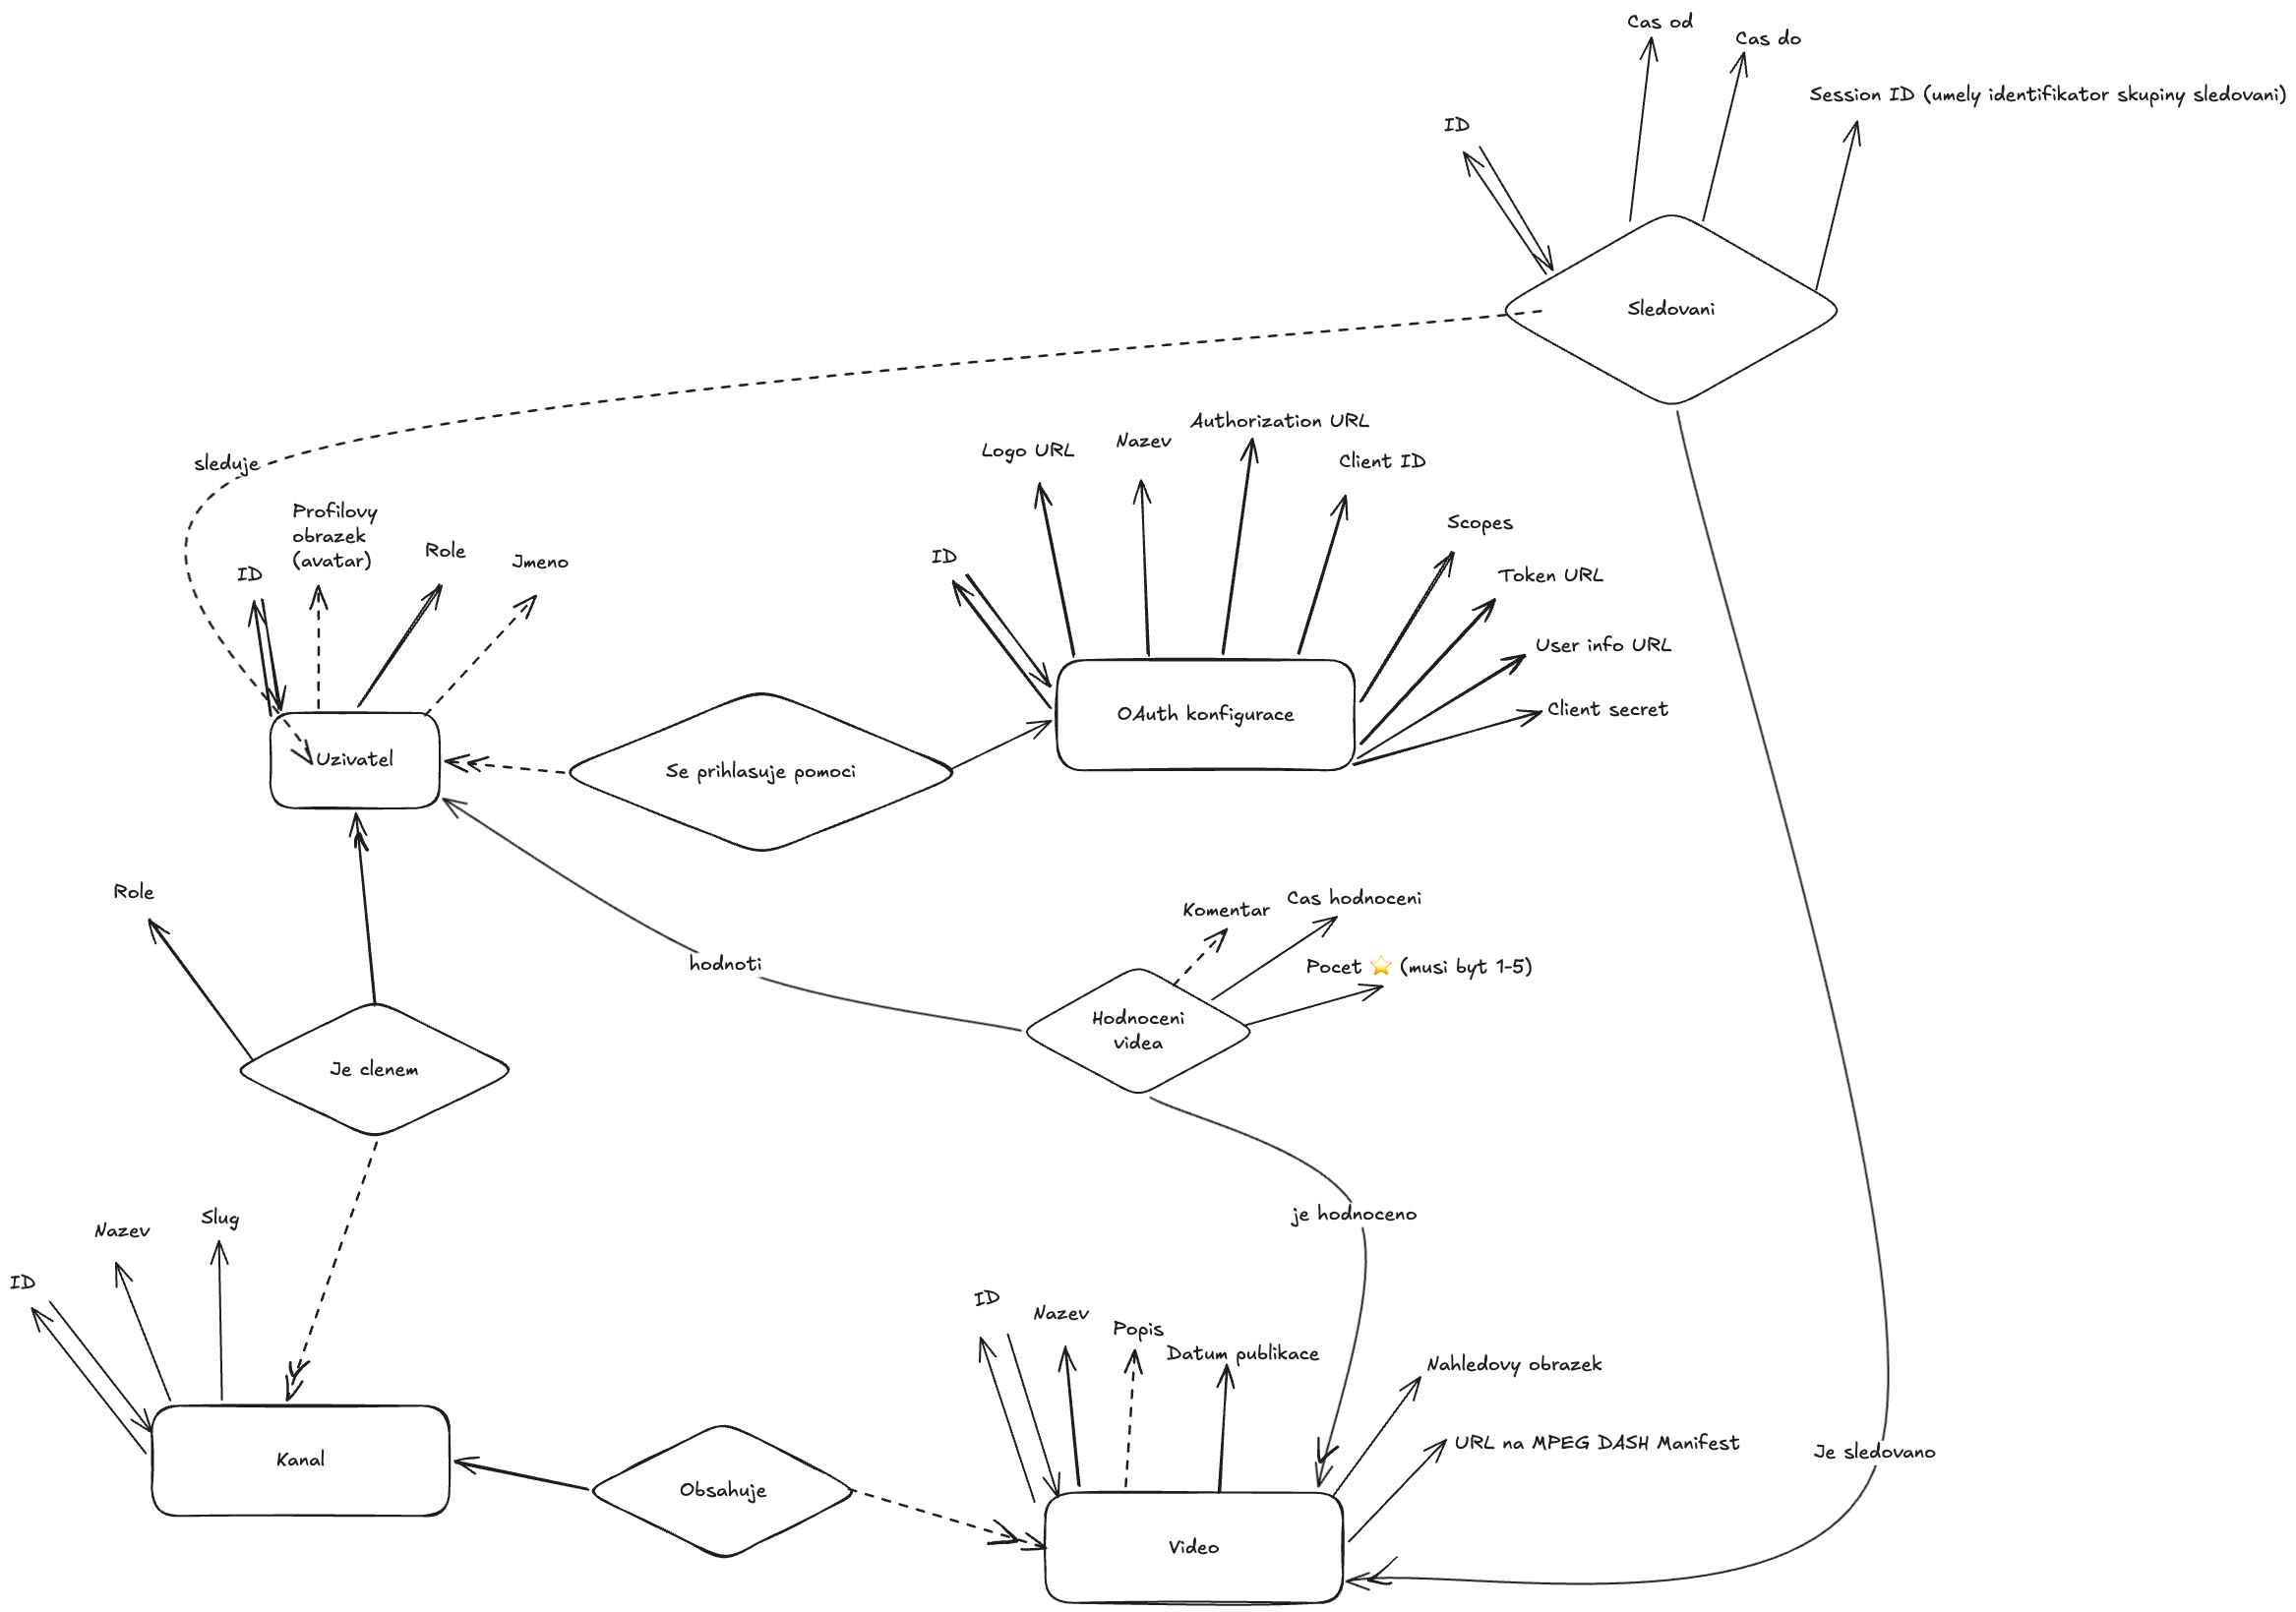
\includegraphics[width=\textwidth]{conceptual-model.png}
\caption{Konceptuální schéma reality -- Platforma na publikování a sledování amatérských filmů}
\end{figure}

\newpage

% ====================================================================
% 3. KONCEPTUÁLNÍ DATOVÝ MODEL
% ====================================================================
\section{Konceptuální datový model}

\begin{figure}[H]
\centering
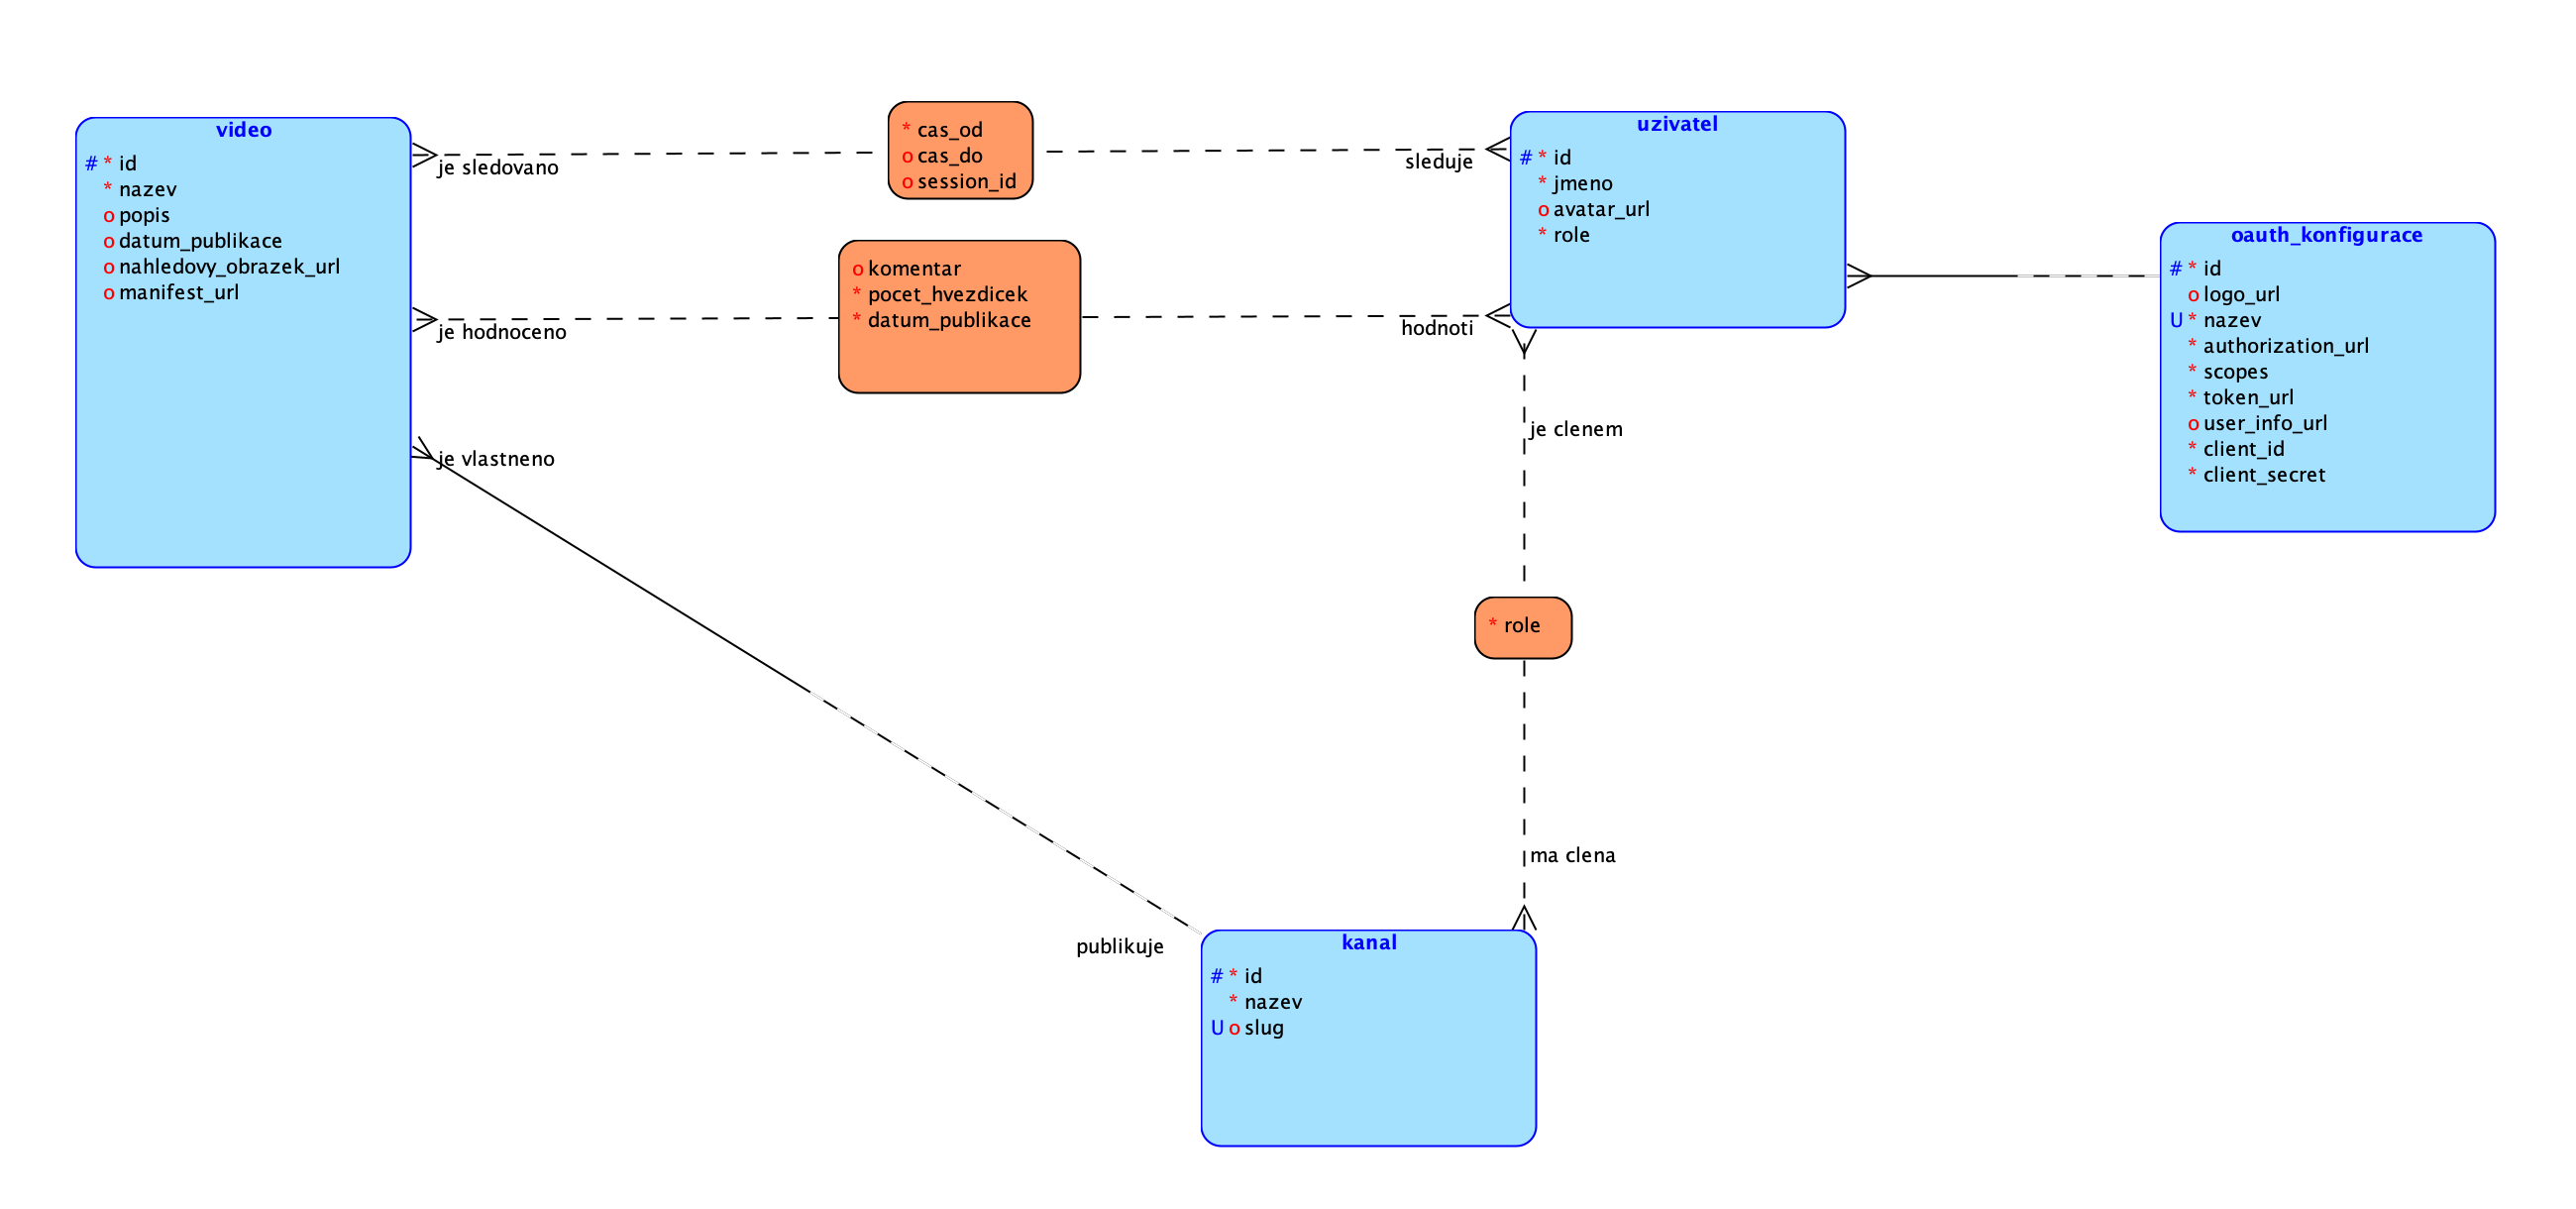
\includegraphics[width=\textwidth]{logical-model.png}
\caption{Konceptuální datový model -- výstup z~CASE nástroje}
\end{figure}

\newpage

% ====================================================================
% 4. DOKUMENTACE DATABÁZE
% ====================================================================
\section{Dokumentace databáze}

\subsection{Fyzický datový model}

\begin{figure}[H]
\centering
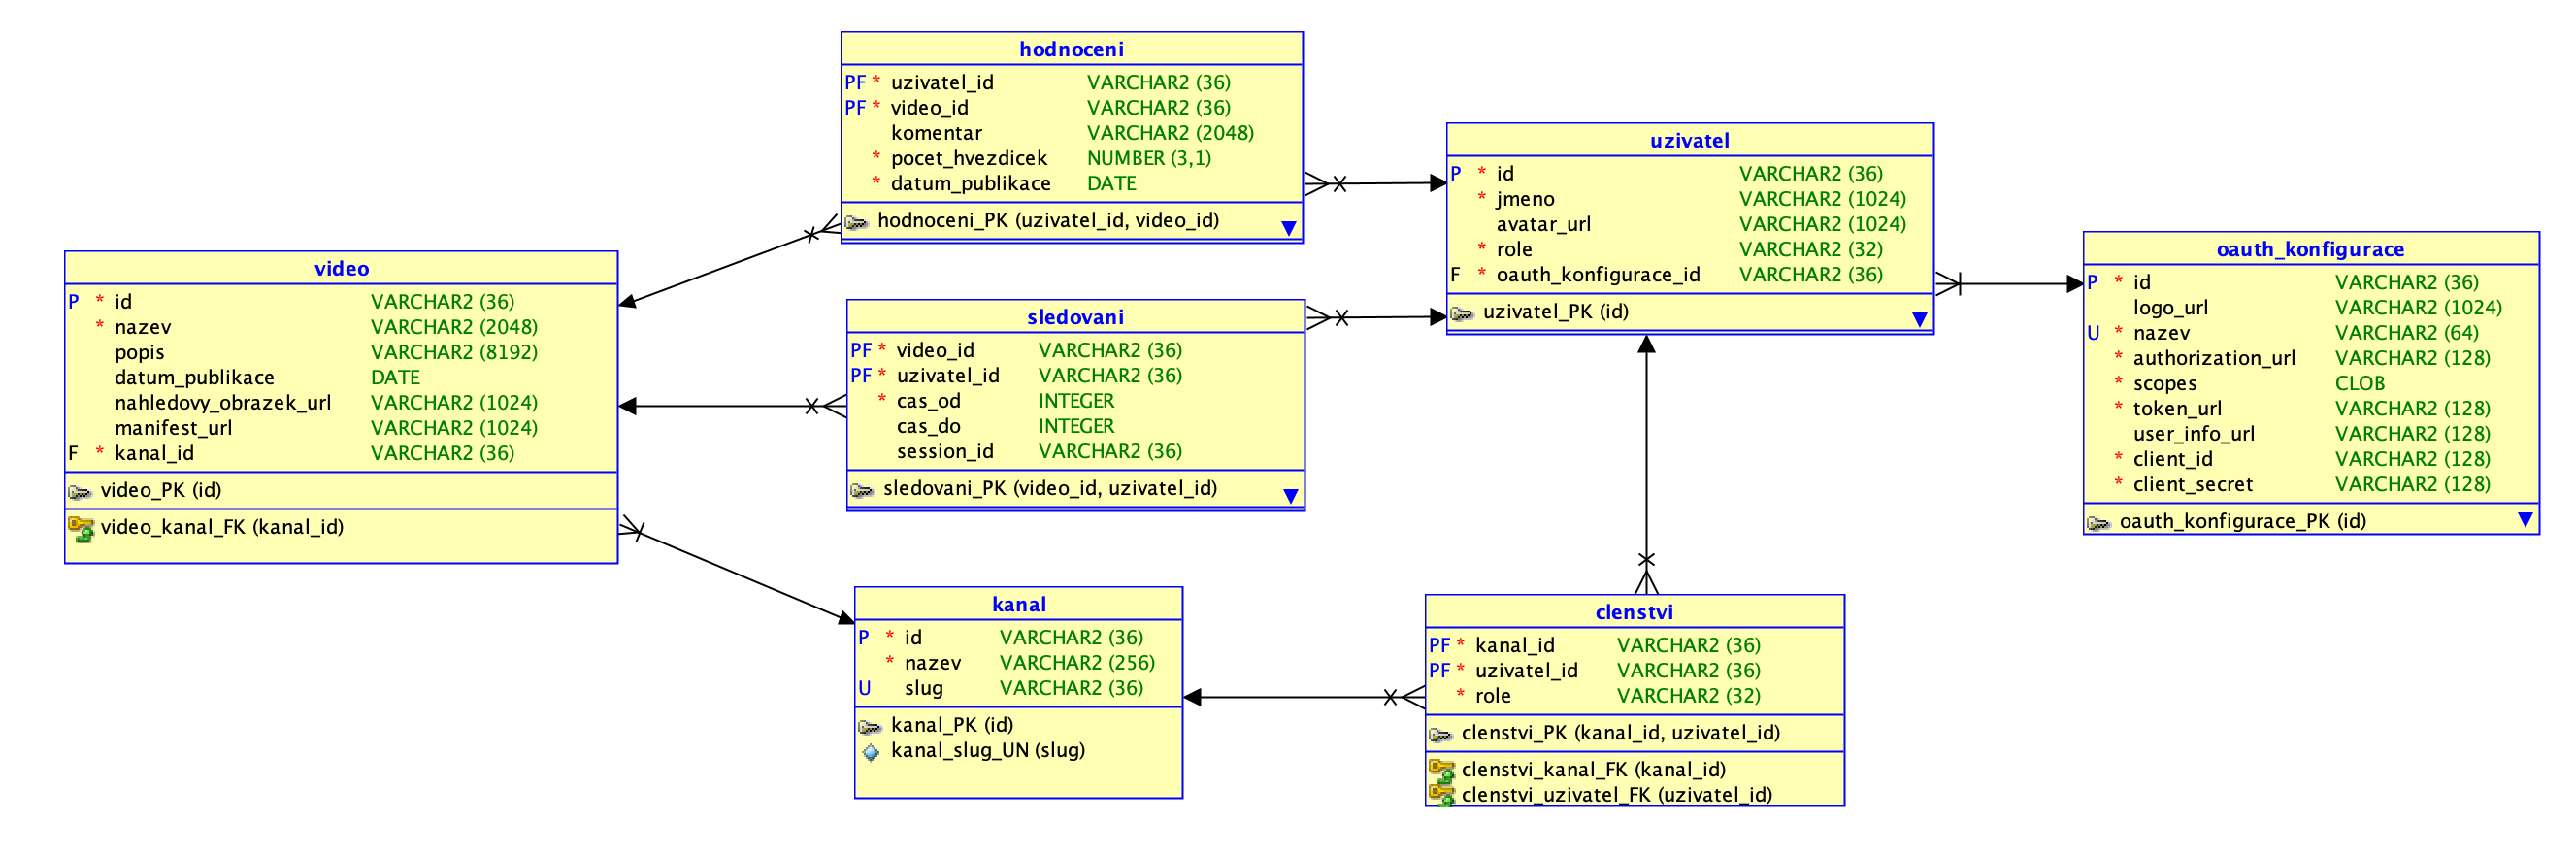
\includegraphics[width=\textwidth]{physical-model.png}
\caption{Fyzický datový model -- výstup z~CASE nástroje}
\end{figure}

\newpage

% ---- 4.2 DEFINICE RELAČNÍCH TABULEK ----
\subsection{Definice relačních tabulek a souvisejících objektů}

Následující SQL příkazy byly vygenerovány nástrojem Oracle SQL Developer Data Modeler a~doplněny o~příkazy pro definici přístupových práv.

\begin{lstlisting}
-- Generated by Oracle SQL Developer Data Modeler 24.3.1.351.0831
--   at:        2026-05-14 00:46:09 CEST
--   site:      Oracle Database 11g
--   type:      Oracle Database 11g

CREATE TABLE clenstvi
    (
     kanal_id    VARCHAR2 (36)  NOT NULL ,
     uzivatel_id VARCHAR2 (36)  NOT NULL ,
     role        VARCHAR2 (32)  NOT NULL
    )
;

ALTER TABLE clenstvi
    ADD
    CHECK (role IN ('admin', 'clen'))
;

ALTER TABLE clenstvi
    ADD CONSTRAINT clenstvi_PK
    PRIMARY KEY ( kanal_id, uzivatel_id ) ;

CREATE TABLE hodnoceni
    (
     uzivatel_id     VARCHAR2 (36)  NOT NULL ,
     video_id        VARCHAR2 (36)  NOT NULL ,
     komentar        VARCHAR2 (2048) ,
     pocet_hvezdicek NUMBER (3,1)  NOT NULL ,
     datum_publikace DATE  NOT NULL
    )
;

ALTER TABLE hodnoceni
    ADD
    CHECK (pocet_hvezdicek IN
      (1, 1.5, 2, 2.5, 3, 3.5, 4, 4.5, 5))
;

ALTER TABLE hodnoceni
    ADD CONSTRAINT hodnoceni_PK
    PRIMARY KEY ( uzivatel_id, video_id ) ;

CREATE TABLE kanal
    (
     id    VARCHAR2 (36)  NOT NULL ,
     nazev VARCHAR2 (256)  NOT NULL ,
     slug  VARCHAR2 (36)
    )
;

ALTER TABLE kanal
    ADD CONSTRAINT kanal_PK PRIMARY KEY ( id ) ;

ALTER TABLE kanal
    ADD CONSTRAINT kanal_slug_UN UNIQUE ( slug ) ;
\end{lstlisting}

\begin{lstlisting}
CREATE TABLE oauth_konfigurace
    (
     id                VARCHAR2 (36)  NOT NULL ,
     logo_url          VARCHAR2 (1024) ,
     nazev             VARCHAR2 (64)  NOT NULL ,
     authorization_url VARCHAR2 (128)  NOT NULL ,
     scopes            CLOB  NOT NULL ,
     token_url         VARCHAR2 (128)  NOT NULL ,
     user_info_url     VARCHAR2 (128) ,
     client_id         VARCHAR2 (128)  NOT NULL ,
     client_secret     VARCHAR2 (128)  NOT NULL
    )
;

ALTER TABLE oauth_konfigurace
    ADD CONSTRAINT oauth_konfigurace_PK
    PRIMARY KEY ( id ) ;

ALTER TABLE oauth_konfigurace
    ADD CONSTRAINT oauth_konfigurace_nazev_UN
    UNIQUE ( nazev ) ;

CREATE TABLE sledovani
    (
     video_id    VARCHAR2 (36)  NOT NULL ,
     uzivatel_id VARCHAR2 (36)  NOT NULL ,
     id          VARCHAR2 (36)  NOT NULL ,
     cas_od      INTEGER  NOT NULL ,
     cas_do      INTEGER ,
     session_id  VARCHAR2 (36)
    )
;

ALTER TABLE sledovani
    ADD CONSTRAINT sledovani_PK
    PRIMARY KEY ( id ) ;

CREATE TABLE uzivatel
    (
     id                   VARCHAR2 (36)  NOT NULL ,
     jmeno                VARCHAR2 (1024)  NOT NULL ,
     avatar_url           VARCHAR2 (1024) ,
     role                 VARCHAR2 (32)  NOT NULL ,
     oauth_konfigurace_id VARCHAR2 (36)  NOT NULL
    )
;

ALTER TABLE uzivatel
    ADD
    CHECK (role IN ('admin', 'uzivatel'))
;

ALTER TABLE uzivatel
    ADD CONSTRAINT uzivatel_PK PRIMARY KEY ( id ) ;
\end{lstlisting}

\begin{lstlisting}
CREATE TABLE video
    (
     id                    VARCHAR2 (36)  NOT NULL ,
     nazev                 VARCHAR2 (2048)  NOT NULL ,
     popis                 VARCHAR2 (8192) ,
     datum_publikace       DATE ,
     nahledovy_obrazek_url VARCHAR2 (1024) ,
     manifest_url          VARCHAR2 (1024) ,
     kanal_id              VARCHAR2 (36)  NOT NULL
    )
;

ALTER TABLE video
    ADD CONSTRAINT video_PK PRIMARY KEY ( id ) ;

/*==============================================================*/
/* Foreign Keys                                                 */
/*==============================================================*/

ALTER TABLE clenstvi
    ADD CONSTRAINT clenstvi_kanal_FK FOREIGN KEY
    ( kanal_id )
    REFERENCES kanal ( id )
    ON DELETE CASCADE
;

ALTER TABLE clenstvi
    ADD CONSTRAINT clenstvi_uzivatel_FK FOREIGN KEY
    ( uzivatel_id )
    REFERENCES uzivatel ( id )
    ON DELETE CASCADE
;

ALTER TABLE hodnoceni
    ADD CONSTRAINT hodnoceni_uzivatel_FK FOREIGN KEY
    ( uzivatel_id )
    REFERENCES uzivatel ( id )
    ON DELETE CASCADE
;

ALTER TABLE hodnoceni
    ADD CONSTRAINT hodnoceni_video_FK FOREIGN KEY
    ( video_id )
    REFERENCES video ( id )
    ON DELETE CASCADE
;

ALTER TABLE sledovani
    ADD CONSTRAINT sledovani_uzivatel_FK FOREIGN KEY
    ( uzivatel_id )
    REFERENCES uzivatel ( id )
    ON DELETE CASCADE
;

ALTER TABLE sledovani
    ADD CONSTRAINT sledovani_video_FK FOREIGN KEY
    ( video_id )
    REFERENCES video ( id )
    ON DELETE CASCADE
;

ALTER TABLE uzivatel
    ADD CONSTRAINT uzivatel_oauth_konfigurace_FK
    FOREIGN KEY ( oauth_konfigurace_id )
    REFERENCES oauth_konfigurace ( id )
;

ALTER TABLE video
    ADD CONSTRAINT video_kanal_FK FOREIGN KEY
    ( kanal_id )
    REFERENCES kanal ( id )
;
\end{lstlisting}

\newpage

% ---- 4.3 INTEGRITNÍ OMEZENÍ ----
\subsection{Integritní omezení}

\subsubsection{Tabulka OAUTH\_KONFIGURACE}

\paragraph{Entitní integrita}
Atributy tvořící primární klíč: \texttt{ID}

SQL kód pro definici primárního klíče:
\begin{lstlisting}
ALTER TABLE oauth_konfigurace
    ADD CONSTRAINT oauth_konfigurace_PK
    PRIMARY KEY ( id ) ;
\end{lstlisting}

\paragraph{Doménová integrita}

\textbf{Název poskytovatele musí být unikátní}

Popis omezení: Každý poskytovatel identity má unikátní název (např. Google, GitHub), aby
nedocházelo k~duplicitním konfiguracím.

SQL kód příslušného omezení:
\begin{lstlisting}
ALTER TABLE oauth_konfigurace
    ADD CONSTRAINT oauth_konfigurace_nazev_UN
    UNIQUE ( nazev ) ;
\end{lstlisting}

\paragraph{Referenční integrita}
V~tabulce oauth\_konfigurace žádný ze sloupců nepředstavuje cizí klíč.

% ---- UZIVATEL ----
\subsubsection{Tabulka UZIVATEL}

\paragraph{Entitní integrita}
Atributy tvořící primární klíč: \texttt{ID}

SQL kód pro definici primárního klíče:
\begin{lstlisting}
ALTER TABLE uzivatel
    ADD CONSTRAINT uzivatel_PK PRIMARY KEY ( id ) ;
\end{lstlisting}

\paragraph{Doménová integrita}

\textbf{Role uživatele musí být \texttt{'admin'} nebo \texttt{'uzivatel'}}

Popis omezení: Každý uživatel platformy má přiřazenu jednu ze dvou rolí. Jiné hodnoty
nejsou přípustné.

SQL kód příslušného omezení:
\begin{lstlisting}
ALTER TABLE uzivatel
    ADD
    CHECK (role IN ('admin', 'uzivatel'))
;
\end{lstlisting}

\paragraph{Referenční integrita}

\textbf{Sloupec oauth\_konfigurace\_id v~tabulce uzivatel představuje cizí klíč}

Popis omezení: Každý uživatel se přihlašuje prostřednictvím právě jednoho externího
poskytovatele identity. Sloupec oauth\_konfigurace\_id obsahuje identifikátor příslušné
OAuth konfigurace.

Druh použitého řešení referenční integrity pro operaci DELETE: RESTRICT.

SQL kód příslušného omezení:
\begin{lstlisting}
ALTER TABLE uzivatel
    ADD CONSTRAINT uzivatel_oauth_konfigurace_FK
    FOREIGN KEY ( oauth_konfigurace_id )
    REFERENCES oauth_konfigurace ( id )
;
\end{lstlisting}
Pozn.: Nelze smazat OAuth konfiguraci, pokud existují uživatelé, kteří ji používají.

% ---- KANAL ----
\subsubsection{Tabulka KANAL}

\paragraph{Entitní integrita}
Atributy tvořící primární klíč: \texttt{ID}

SQL kód pro definici primárního klíče:
\begin{lstlisting}
ALTER TABLE kanal
    ADD CONSTRAINT kanal_PK PRIMARY KEY ( id ) ;
\end{lstlisting}

\paragraph{Doménová integrita}

\textbf{Slug kanálu musí být unikátní (pokud je uveden)}

Popis omezení: Slug slouží jako URL-přátelský identifikátor kanálu. Pokud je uveden, musí
být v~rámci platformy jednoznačný. Hodnota NULL je povolena (slug je volitelný).

SQL kód příslušného omezení:
\begin{lstlisting}
ALTER TABLE kanal
    ADD CONSTRAINT kanal_slug_UN UNIQUE ( slug ) ;
\end{lstlisting}
Pozn.: Oracle UNIQUE constraint povoluje více NULL hodnot.

\paragraph{Referenční integrita}
V~tabulce kanal žádný ze sloupců nepředstavuje cizí klíč.

% ---- CLENSTVI ----
\subsubsection{Tabulka CLENSTVI}

\paragraph{Entitní integrita}
Atributy tvořící primární klíč: \texttt{KANAL\_ID}, \texttt{UZIVATEL\_ID}

SQL kód pro definici primárního klíče:
\begin{lstlisting}
ALTER TABLE clenstvi
    ADD CONSTRAINT clenstvi_PK
    PRIMARY KEY ( kanal_id, uzivatel_id ) ;
\end{lstlisting}
Pozn.: Složený primární klíč zajišťuje, že jeden uživatel může být členem daného kanálu
nejvýše jednou.

\paragraph{Doménová integrita}

\textbf{Role člena kanálu musí být jedna z~definovaných hodnot}

Popis omezení: V~každém kanálu má uživatel přiřazenu právě jednu roli. Přípustné hodnoty
jsou \texttt{'admin'} a~\texttt{'clen'}.

SQL kód příslušného omezení:
\begin{lstlisting}
ALTER TABLE clenstvi
    ADD
    CHECK (role IN ('admin', 'clen'))
;
\end{lstlisting}

\paragraph{Referenční integrita}

\textbf{Sloupec kanal\_id v~tabulce clenstvi představuje cizí klíč}

Popis omezení: Tabulka clenstvi realizuje vztah M:N mezi entitními množinami Uživatel
a~Kanál. Sloupec kanal\_id identifikuje kanál.

Druh použitého řešení referenční integrity pro operaci DELETE: CASCADE.

SQL kód příslušného omezení:
\begin{lstlisting}
ALTER TABLE clenstvi
    ADD CONSTRAINT clenstvi_kanal_FK FOREIGN KEY
    ( kanal_id )
    REFERENCES kanal ( id )
    ON DELETE CASCADE
;
\end{lstlisting}
Pozn.: Při smazání kanálu se automaticky smažou i~záznamy o~členství.

\textbf{Sloupec uzivatel\_id v~tabulce clenstvi představuje cizí klíč}

Popis omezení: Sloupec uzivatel\_id identifikuje uživatele, který je členem kanálu.

Druh použitého řešení referenční integrity pro operaci DELETE: CASCADE.

SQL kód příslušného omezení:
\begin{lstlisting}
ALTER TABLE clenstvi
    ADD CONSTRAINT clenstvi_uzivatel_FK FOREIGN KEY
    ( uzivatel_id )
    REFERENCES uzivatel ( id )
    ON DELETE CASCADE
;
\end{lstlisting}
Pozn.: Při smazání uživatele se automaticky smažou i~záznamy o~jeho členství.

% ---- VIDEO ----
\subsubsection{Tabulka VIDEO}

\paragraph{Entitní integrita}
Atributy tvořící primární klíč: \texttt{ID}

SQL kód pro definici primárního klíče:
\begin{lstlisting}
ALTER TABLE video
    ADD CONSTRAINT video_PK PRIMARY KEY ( id ) ;
\end{lstlisting}

\paragraph{Doménová integrita}
V~rámci tabulky video nejsou definována žádná omezení sloužící k~zajištění doménové
integrity nad rámec NOT NULL omezení sloupce nazev.

\paragraph{Referenční integrita}

\textbf{Sloupec kanal\_id v~tabulce video představuje cizí klíč}

Popis omezení: Každé video je vlastněno právě jedním kanálem. Sloupec kanal\_id
identifikuje kanál, do kterého video náleží.

Druh použitého řešení referenční integrity pro operaci DELETE: RESTRICT.

SQL kód příslušného omezení:
\begin{lstlisting}
ALTER TABLE video
    ADD CONSTRAINT video_kanal_FK FOREIGN KEY
    ( kanal_id )
    REFERENCES kanal ( id )
;
\end{lstlisting}
Pozn.: Nelze smazat kanál, pokud obsahuje videa. Videa je třeba nejprve smazat nebo
přesunout do jiného kanálu.

% ---- HODNOCENI ----
\subsubsection{Tabulka HODNOCENI}

\paragraph{Entitní integrita}
Atributy tvořící primární klíč: \texttt{UZIVATEL\_ID}, \texttt{VIDEO\_ID}

SQL kód pro definici primárního klíče:
\begin{lstlisting}
ALTER TABLE hodnoceni
    ADD CONSTRAINT hodnoceni_PK
    PRIMARY KEY ( uzivatel_id, video_id ) ;
\end{lstlisting}
Pozn.: Složený primární klíč zajišťuje, že jeden uživatel může hodnotit dané video
nejvýše jednou.

\paragraph{Doménová integrita}

\textbf{Počet hvězdiček musí být jedna z~přípustných hodnot 1 až 5 (včetně polovičních)}

Popis omezení: Hodnocení videa je vyjádřeno číselnou hodnotou. Přípustné jsou celočíselné
hodnoty a~jejich poloviny: 1; 1,5; 2; 2,5; 3; 3,5; 4; 4,5; 5.

SQL kód příslušného omezení:
\begin{lstlisting}
ALTER TABLE hodnoceni
    ADD
    CHECK (pocet_hvezdicek IN
      (1, 1.5, 2, 2.5, 3, 3.5, 4, 4.5, 5))
;
\end{lstlisting}
Pozn.: Datový typ NUMBER(3,1) zajišťuje přesnost na jedno desetinné místo.

\paragraph{Referenční integrita}

\textbf{Sloupec uzivatel\_id v~tabulce hodnoceni představuje cizí klíč}

Popis omezení: Hodnocení je vázáno na jednoho uživatele.

Druh použitého řešení referenční integrity pro operaci DELETE: CASCADE.

SQL kód příslušného omezení:
\begin{lstlisting}
ALTER TABLE hodnoceni
    ADD CONSTRAINT hodnoceni_uzivatel_FK FOREIGN KEY
    ( uzivatel_id )
    REFERENCES uzivatel ( id )
    ON DELETE CASCADE
;
\end{lstlisting}

\textbf{Sloupec video\_id v~tabulce hodnoceni představuje cizí klíč}

Popis omezení: Hodnocení je vázáno na jedno video.

Druh použitého řešení referenční integrity pro operaci DELETE: CASCADE.

SQL kód příslušného omezení:
\begin{lstlisting}
ALTER TABLE hodnoceni
    ADD CONSTRAINT hodnoceni_video_FK FOREIGN KEY
    ( video_id )
    REFERENCES video ( id )
    ON DELETE CASCADE
;
\end{lstlisting}
Pozn.: Při smazání videa se automaticky smažou i~všechna jeho hodnocení.

% ---- SLEDOVANI ----
\subsubsection{Tabulka SLEDOVANI}

\paragraph{Entitní integrita}
Atributy tvořící primární klíč: \texttt{ID}

SQL kód pro definici primárního klíče:
\begin{lstlisting}
ALTER TABLE sledovani
    ADD CONSTRAINT sledovani_PK
    PRIMARY KEY ( id ) ;
\end{lstlisting}
Pozn.: Umělý identifikátor (UUID) slouží jako primární klíč, protože jeden uživatel může
mít více záznamů o~sledování téhož videa (např. více heartbeatů v~rámci jednoho přehrávání
nebo opakované zhlédnutí).

\paragraph{Doménová integrita}
V~rámci tabulky sledovani nejsou definována žádná omezení sloužící k~zajištění doménové
integrity nad rámec NOT NULL omezení sloupců video\_id, uzivatel\_id, id a~cas\_od.
Sloupce cas\_od a~cas\_do jsou typu INTEGER a~představují pozici v~sekundách od začátku
videa.

\paragraph{Referenční integrita}

\textbf{Sloupec uzivatel\_id v~tabulce sledovani představuje cizí klíč}

Popis omezení: Aktivita sledování je vázána na jednoho uživatele.

Druh použitého řešení referenční integrity pro operaci DELETE: CASCADE\footnote{Alternativní návrh kaskádování po výmazu uživatele spojeného se sledovací aktivitou obsahoval nastavení uživatelského ID záznamu na hodnotu NULL. Bohužel, stejně jako výmaz celého záznamu kaskádovaním s sebou přináší NULL své vlastní mouchy, jako tu, že NULL by omezil možnost rozlišení počtu unikátních uživatelů, kteří video zhlédli.}.

SQL kód příslušného omezení:
\begin{lstlisting}
ALTER TABLE sledovani
    ADD CONSTRAINT sledovani_uzivatel_FK FOREIGN KEY
    ( uzivatel_id )
    REFERENCES uzivatel ( id )
    ON DELETE CASCADE
;
\end{lstlisting}

\textbf{Sloupec video\_id v~tabulce sledovani představuje cizí klíč}

Popis omezení: Aktivita sledování je vázána na jedno video.

Druh použitého řešení referenční integrity pro operaci DELETE: CASCADE.

SQL kód příslušného omezení:
\begin{lstlisting}
ALTER TABLE sledovani
    ADD CONSTRAINT sledovani_video_FK FOREIGN KEY
    ( video_id )
    REFERENCES video ( id )
    ON DELETE CASCADE
;
\end{lstlisting}
Pozn.: Při smazání videa se automaticky smažou i~záznamy o~jeho sledování.

\newpage

% ---- 4.4 DEFINICE PŘÍSTUPOVÝCH PRÁV ----
\subsection{Definice přístupových práv}

Pro uživatele \texttt{STUDENT} jsou definována práva pro operaci SELECT na všech tabulkách.
Pro uživatele \texttt{DB4IT218} jsou definována práva na operace SELECT, INSERT, UPDATE
a~DELETE na všech tabulkách.

\begin{lstlisting}
-- Prava pro uzivatele STUDENT (pouze SELECT)
GRANT SELECT ON oauth_konfigurace TO STUDENT;
GRANT SELECT ON uzivatel TO STUDENT;
GRANT SELECT ON kanal TO STUDENT;
GRANT SELECT ON clenstvi TO STUDENT;
GRANT SELECT ON video TO STUDENT;
GRANT SELECT ON hodnoceni TO STUDENT;
GRANT SELECT ON sledovani TO STUDENT;

-- Prava pro uzivatele DB4IT218 (CRUD)
GRANT SELECT, INSERT, UPDATE, DELETE
  ON oauth_konfigurace TO DB4IT218;
GRANT SELECT, INSERT, UPDATE, DELETE
  ON uzivatel TO DB4IT218;
GRANT SELECT, INSERT, UPDATE, DELETE
  ON kanal TO DB4IT218;
GRANT SELECT, INSERT, UPDATE, DELETE
  ON clenstvi TO DB4IT218;
GRANT SELECT, INSERT, UPDATE, DELETE
  ON video TO DB4IT218;
GRANT SELECT, INSERT, UPDATE, DELETE
  ON hodnoceni TO DB4IT218;
GRANT SELECT, INSERT, UPDATE, DELETE
  ON sledovani TO DB4IT218;
\end{lstlisting}

\newpage

% ---- 4.5 DEFINICE DALŠÍCH DATABÁZOVÝCH OBJEKTŮ ----
\subsection{Definice dalších databázových objektů}

\subsubsection*{Pohledy (Views)}

Pro podporu dotazů uvedených v~zadání jsou vytvořeny následující pohledy:

\textbf{View videa\_v\_kanalu} -- zobrazuje videa patřící do jednotlivých kanálů
(odpovídá na dotaz: \emph{Jaká videa patří ke konkrétnímu kanálu?}):

\begin{lstlisting}
CREATE OR REPLACE VIEW videa_v_kanalu AS
SELECT k.id AS kanal_id,
       k.nazev AS kanal_nazev,
       k.slug,
       v.id AS video_id,
       v.nazev AS video_nazev,
       v.popis,
       v.datum_publikace
FROM kanal k
JOIN video v ON v.kanal_id = k.id
ORDER BY k.nazev, v.datum_publikace DESC;

GRANT SELECT ON videa_v_kanalu TO STUDENT;
GRANT SELECT ON videa_v_kanalu TO DB4IT218;
\end{lstlisting}

\textbf{View hodnoceni\_videi} -- zobrazuje souhrnné hodnocení jednotlivých videí
(odpovídá na dotaz: \emph{Jak je dané video hodnoceno?}):

\begin{lstlisting}
CREATE OR REPLACE VIEW hodnoceni_videi AS
SELECT v.id AS video_id,
       v.nazev AS video_nazev,
       COUNT(h.uzivatel_id) AS pocet_hodnoceni,
       ROUND(AVG(h.pocet_hvezdicek), 1)
         AS prumerne_hodnoceni,
       MIN(h.pocet_hvezdicek) AS min_hodnoceni,
       MAX(h.pocet_hvezdicek) AS max_hodnoceni
FROM video v
LEFT JOIN hodnoceni h ON h.video_id = v.id
GROUP BY v.id, v.nazev;

GRANT SELECT ON hodnoceni_videi TO STUDENT;
GRANT SELECT ON hodnoceni_videi TO DB4IT218;
\end{lstlisting}

\textbf{View clenove\_kanalu} -- zobrazuje členy kanálů a~jejich role
(odpovídá na dotaz: \emph{Kdo je členem kanálu a~jakou v~něm má roli?}):

\begin{lstlisting}
CREATE OR REPLACE VIEW clenove_kanalu AS
SELECT k.id AS kanal_id,
       k.nazev AS kanal_nazev,
       u.id AS uzivatel_id,
       u.jmeno,
       c.role
FROM kanal k
JOIN clenstvi c ON c.kanal_id = k.id
JOIN uzivatel u ON u.id = c.uzivatel_id
ORDER BY k.nazev, c.role, u.jmeno;

GRANT SELECT ON clenove_kanalu TO STUDENT;
GRANT SELECT ON clenove_kanalu TO DB4IT218;
\end{lstlisting}

\newpage

% ====================================================================
% 5. OBSAH DATABÁZE
% ====================================================================
\section{Obsah databáze}

\subsection{SQL příkazy pro naplnění databáze daty}
\label{sec:insert}

\begin{lstlisting}
-- 1. OAUTH KONFIGURACE
INSERT INTO oauth_konfigurace (id, logo_url, nazev,
  authorization_url, scopes, token_url, user_info_url,
  client_id, client_secret)
VALUES ('00b3f810-0000-7abc-8def-000000001998',
  'https://upload.wikimedia.org/wikipedia/commons/c/c1/Google_%22G%22_logo.svg',
  'Google',
  'https://accounts.google.com/o/oauth2/v2/auth',
  'openid profile',
  'https://oauth2.googleapis.com/token',
  'https://openidconnect.googleapis.com/v1/userinfo',
  'client-id-1', 'secret-1');

INSERT INTO oauth_konfigurace (id, logo_url, nazev,
  authorization_url, scopes, token_url, user_info_url,
  client_id, client_secret)
VALUES ('0119e830-0000-7abc-8def-000000002008',
  'https://github.githubassets.com/images/modules/logos_page/GitHub-Mark.png',
  'GitHub',
  'https://github.com/login/oauth/authorize',
  'read:user',
  'https://github.com/login/oauth/access_token',
  'https://api.github.com/user',
  'client-id-2', 'secret-2');

INSERT INTO oauth_konfigurace (id, logo_url, nazev,
  authorization_url, scopes, token_url, user_info_url,
  client_id, client_secret)
VALUES ('014c2b90-0000-7abc-8def-000000002015',
  'https://upload.wikimedia.org/wikipedia/commons/3/3c/Discord_Color_Text_Logo.svg',
  'Discord',
  'https://discord.com/api/oauth2/authorize',
  'identify email',
  'https://discord.com/api/oauth2/token',
  'https://discord.com/api/users/@me',
  'client-id-3', 'secret-3');
\end{lstlisting}

\begin{lstlisting}
-- 2. KANAL
INSERT INTO kanal (id, nazev, slug)
VALUES ('011409f0-0000-7abc-8def-000000002015',
  'TagTram Studios', 'tagtram-studios');

INSERT INTO kanal (id, nazev, slug)
VALUES ('00f074d0-0000-7abc-8def-000000002012',
  'A24 films', 'a24-films');

INSERT INTO kanal (id, nazev, slug)
VALUES ('00c0a310-0000-7abc-8def-000000001989',
  'Televizní vysílání Malín', 'tv-malin');
\end{lstlisting}

\begin{lstlisting}
-- 3. UZIVATEL
INSERT INTO uzivatel (id, jmeno, avatar_url, role,
  oauth_konfigurace_id)
VALUES ('02d98d5b-1880-7abc-8def-000000002069',
  'Filip Filmíček',
  'https://ui-avatars.com/api/?name=Filip+Filmicek&background=random',
  'uzivatel',
  '00b3f810-0000-7abc-8def-000000001998');

INSERT INTO uzivatel (id, jmeno, avatar_url, role,
  oauth_konfigurace_id)
VALUES ('03459ebd-e000-7abc-8def-000000002084',
  'Eas Anderson',
  'https://ui-avatars.com/api/?name=Eas+Anderson&background=random',
  'uzivatel',
  '00b3f810-0000-7abc-8def-000000001998');

INSERT INTO uzivatel (id, jmeno, avatar_url, role,
  oauth_konfigurace_id)
VALUES ('04cb2204-0000-7abc-8def-000000002137',
  'Jirka Kosek',
  'https://ui-avatars.com/api/?name=Jirka+Kosek&background=random',
  'admin',
  '0119e830-0000-7abc-8def-000000002008');

INSERT INTO uzivatel (id, jmeno, avatar_url, role,
  oauth_konfigurace_id)
VALUES ('0e608a7c-6bff-7abc-8def-000000009999',
  'Ing. Pavel Vedral',
  'https://ui-avatars.com/api/?name=Pavel+Vedral&background=random',
  'uzivatel',
  '0119e830-0000-7abc-8def-000000002008');

INSERT INTO uzivatel (id, jmeno, avatar_url, role,
  oauth_konfigurace_id)
VALUES ('00dc5895-bfff-7abc-8def-000000001999',
  'Ing. Dušan Chlapek, Ph.D.',
  'https://ui-avatars.com/api/?name=Dusan+Chlapek&background=random',
  'uzivatel',
  '014c2b90-0000-7abc-8def-000000002015');
\end{lstlisting}

\begin{lstlisting}
-- 4. CLENSTVI
INSERT INTO clenstvi (kanal_id, uzivatel_id, role)
VALUES ('011409f0-0000-7abc-8def-000000002015',
  '04cb2204-0000-7abc-8def-000000002137', 'admin');

INSERT INTO clenstvi (kanal_id, uzivatel_id, role)
VALUES ('00f074d0-0000-7abc-8def-000000002012',
  '0e608a7c-6bff-7abc-8def-000000009999', 'clen');

INSERT INTO clenstvi (kanal_id, uzivatel_id, role)
VALUES ('00c0a310-0000-7abc-8def-000000001989',
  '00dc5895-bfff-7abc-8def-000000001999', 'admin');
\end{lstlisting}

\begin{lstlisting}
-- 5. VIDEO
INSERT INTO video (id, nazev, popis, datum_publikace,
  nahledovy_obrazek_url, manifest_url, kanal_id)
VALUES ('019159d0-0000-7abc-8def-000000002025',
  'Krátkodobé řešení',
  'Vždy si jděte za svými sny.',
  DATE '2025-06-15',
  'https://picsum.photos/seed/kratkodobe/1280/720',
  'https://dash.akamaized.net/akamai/bbb_30fps/bbb_30fps.mpd',
  '011409f0-0000-7abc-8def-000000002015');

INSERT INTO video (id, nazev, popis, datum_publikace,
  nahledovy_obrazek_url, manifest_url, kanal_id)
VALUES ('01947b10-0000-7abc-8def-000000002026',
  'Drama', 'Je to lepší než Backrooms.',
  DATE '2026-01-10',
  'https://picsum.photos/seed/drama/1280/720',
  'https://media.axinom.com/clear/Manifest.mpd',
  '00f074d0-0000-7abc-8def-000000002012');

INSERT INTO video (id, nazev, popis, datum_publikace,
  nahledovy_obrazek_url, manifest_url, kanal_id)
VALUES ('019159d0-1111-7abc-8def-000000002025',
  'Král Žito', 'Pohádka, trochu delší než je třeba.',
  DATE '2025-11-05',
  'https://picsum.photos/seed/zito/1280/720',
  'https://bitmovin-a.akamaihd.net/content/MI201109210084_1/mpds/f08e80da-bf1d-4e3d-8899-f0f6155f6efa.mpd',
  '00c0a310-0000-7abc-8def-000000001989');
\end{lstlisting}

\begin{lstlisting}
-- 6. HODNOCENI
INSERT INTO hodnoceni (uzivatel_id, video_id, komentar,
  pocet_hvezdicek, datum_publikace)
VALUES ('04cb2204-0000-7abc-8def-000000002137',
  '019159d0-0000-7abc-8def-000000002025',
  'Technicky skvělé, XML validní.', 5,
  DATE '2025-06-16');

INSERT INTO hodnoceni (uzivatel_id, video_id, komentar,
  pocet_hvezdicek, datum_publikace)
VALUES ('00dc5895-bfff-7abc-8def-000000001999',
  '01947b10-0000-7abc-8def-000000002026',
  'Chybí tomu jasná ontologie.', 2.5,
  DATE '2026-01-15');

INSERT INTO hodnoceni (uzivatel_id, video_id, komentar,
  pocet_hvezdicek, datum_publikace)
VALUES ('0e608a7c-6bff-7abc-8def-000000009999',
  '019159d0-1111-7abc-8def-000000002025',
  'Jiří Brdečka uvařil.', 4,
  DATE '2025-11-10');

INSERT INTO hodnoceni (uzivatel_id, video_id, komentar,
  pocet_hvezdicek, datum_publikace)
VALUES ('02d98d5b-1880-7abc-8def-000000002069',
  '01947b10-0000-7abc-8def-000000002026',
  NULL, 5, DATE '2026-02-01');

INSERT INTO hodnoceni (uzivatel_id, video_id, komentar,
  pocet_hvezdicek, datum_publikace)
VALUES ('03459ebd-e000-7abc-8def-000000002084',
  '019159d0-0000-7abc-8def-000000002025',
  NULL, 4.5, DATE '2025-06-20');
\end{lstlisting}

\begin{lstlisting}
-- 7. SLEDOVANI
INSERT INTO sledovani (video_id, uzivatel_id, id,
  cas_od, cas_do, session_id)
VALUES ('01947b10-0000-7abc-8def-000000002026',
  '02d98d5b-1880-7abc-8def-000000002069',
  'a0000000-0000-7abc-8def-000000000001',
  0, 7200,
  '00000000-0000-7abc-8def-000000000001');

INSERT INTO sledovani (video_id, uzivatel_id, id,
  cas_od, cas_do, session_id)
VALUES ('01947b10-0000-7abc-8def-000000002026',
  '03459ebd-e000-7abc-8def-000000002084',
  'a0000000-0000-7abc-8def-000000000002',
  120, 7200,
  '00000000-0000-7abc-8def-000000000002');

INSERT INTO sledovani (video_id, uzivatel_id, id,
  cas_od, cas_do, session_id)
VALUES ('019159d0-0000-7abc-8def-000000002025',
  '04cb2204-0000-7abc-8def-000000002137',
  'a0000000-0000-7abc-8def-000000000003',
  0, 1500,
  '00000000-0000-7abc-8def-000000000003');

INSERT INTO sledovani (video_id, uzivatel_id, id,
  cas_od, cas_do, session_id)
VALUES ('019159d0-1111-7abc-8def-000000002025',
  '0e608a7c-6bff-7abc-8def-000000009999',
  'a0000000-0000-7abc-8def-000000000004',
  0, 3600,
  '00000000-0000-7abc-8def-000000000004');

INSERT INTO sledovani (video_id, uzivatel_id, id,
  cas_od, cas_do, session_id)
VALUES ('019159d0-1111-7abc-8def-000000002025',
  '00dc5895-bfff-7abc-8def-000000001999',
  'a0000000-0000-7abc-8def-000000000005',
  0, 300,
  '00000000-0000-7abc-8def-000000000005');

COMMIT;
\end{lstlisting}

\newpage

% ---- 5.2 OPIS VLOŽENÝCH DAT ----
\subsection{Opis vložených dat}

V~následujících tabulkách jsou hodnoty UUID zkráceny na posledních 6 znaků
(prefix \texttt{…}) z~důvodu šířky tabulky. Kompletní hodnoty jsou uvedeny
v~INSERT příkazech v~kapitole~\ref{sec:insert}. Ze stejného důvodu jsou sloupce obsahující URL adresy
(logo\_url, avatar\_url, nahledovy\_obrazek\_url, manifest\_url apod.) vynechány také.

\subsubsection{Tabulka oauth\_konfigurace}

{%
\small\centering
\begin{tabular}{|l|l|l|l|l|}
\hline
\textbf{id} & \textbf{nazev} & \textbf{scopes} & \textbf{client\_id} & \textbf{client\_secret} \\
\hline
…001998 & Google  & openid profile & client-id-1 & secret-1 \\
\hline
…002008 & GitHub  & read:user      & client-id-2 & secret-2 \\
\hline
…002015 & Discord & identify email & client-id-3 & secret-3 \\
\hline
\end{tabular}
\par}

\noindent\textit{Pozn.: Sloupce logo\_url, authorization\_url, token\_url a~user\_info\_url
vynechány -- obsahují URL adresy. Kompletní hodnoty viz INSERT příkazy v~kap.~\ref{sec:insert}.}

\subsubsection{Tabulka uzivatel}

{%
\small\centering
\begin{tabular}{|l|l|l|l|}
\hline
\textbf{id} & \textbf{jmeno} & \textbf{role} & \textbf{oauth\_konfigurace\_id} \\
\hline
…002069 & Filip Filmíček            & uzivatel & …001998 \\
\hline
…002084 & Eas Anderson              & uzivatel & …001998 \\
\hline
…002137 & Jirka Kosek               & admin    & …002008 \\
\hline
…009999 & Ing. Pavel Vedral         & uzivatel & …002008 \\
\hline
…001999 & Ing. Dušan Chlapek, Ph.D. & uzivatel & …002015 \\
\hline
\end{tabular}
\par}

\noindent\textit{Pozn.: Sloupec avatar\_url vynechán -- obsahuje URL adresu.}

\subsubsection{Tabulka kanal}

{%
\small\centering
\begin{tabular}{|l|l|l|}
\hline
\textbf{id} & \textbf{nazev} & \textbf{slug} \\
\hline
…002015 & TagTram Studios          & tagtram-studios \\
\hline
…002012 & A24 films                & a24-films \\
\hline
…001989 & Televizní vysílání Malín & tv-malin \\
\hline
\end{tabular}
\par}

\subsubsection{Tabulka clenstvi}

{%
\small\centering
\begin{tabular}{|l|l|l|}
\hline
\textbf{kanal\_id} & \textbf{uzivatel\_id} & \textbf{role} \\
\hline
…002015 & …002137 & admin \\
\hline
…002012 & …009999 & clen \\
\hline
…001989 & …001999 & admin \\
\hline
\end{tabular}
\par}

\subsubsection{Tabulka video}

{\small
\begin{tabularx}{\textwidth}{|l|l|X|l|l|}
\hline
\textbf{id} & \textbf{nazev} & \textbf{popis} & \textbf{datum\_publikace} & \textbf{kanal\_id} \\
\hline
…002025  & Krátkodobé řešení & Vždy si jděte za svými sny.          & 15-JUN-25 & …002015 \\
\hline
…002026  & Drama             & Je to lepší než Backrooms.           & 10-JAN-26 & …002012 \\
\hline
…002025* & Král Žito         & Pohádka, trochu delší než je třeba.  & 05-NOV-25 & …001989 \\
\hline
\end{tabularx}
}

\noindent\textit{Pozn.: * = id končí na …002025 s~odlišným prefixem (019159d0-1111-…).
Sloupce nahledovy\_obrazek\_url a~manifest\_url vynechány.}

\subsubsection{Tabulka hodnoceni}

{\small
\begin{tabularx}{\textwidth}{|l|l|c|X|l|}
\hline
\textbf{uzivatel\_id} & \textbf{video\_id} & \textbf{$\star$} & \textbf{komentar} & \textbf{datum\_publikace} \\
\hline
…002137 & …002025  & 5   & Technicky skvělé, XML validní.    & 16-JUN-25 \\
\hline
…001999 & …002026  & 2.5 & Chybí tomu jasná ontologie.       & 15-JAN-26 \\
\hline
…009999 & …002025* & 4   & Jiří Brdečka uvařil.   & 10-NOV-25 \\
\hline
…002069 & …002026  & 5   & \textit{NULL}                     & 01-FEB-26 \\
\hline
…002084 & …002025  & 4.5 & \textit{NULL}                     & 20-JUN-25 \\
\hline
\end{tabularx}
}

\subsubsection{Tabulka sledovani}

{\small
\begin{tabularx}{\textwidth}{|l|l|l|r|r|X|}
\hline
\textbf{video\_id} & \textbf{uzivatel\_id} & \textbf{id} & \textbf{cas\_od} & \textbf{cas\_do} & \textbf{session\_id} \\
\hline
…002026  & …002069 & …000001 &   0 & 7200 & …000001 \\
\hline
…002026  & …002084 & …000002 & 120 & 7200 & …000002 \\
\hline
…002025  & …002137 & …000003 &   0 & 1500 & …000003 \\
\hline
…002025* & …009999 & …000004 &   0 & 3600 & …000004 \\
\hline
…002025* & …001999 & …000005 &   0 &  300 & …000005 \\
\hline
\end{tabularx}
}

\end{document}
